\documentclass[a4paper,12pt]{article}
\usepackage{graphicx}
\usepackage{amsmath}
\usepackage{geometry}
\usepackage{float}
\usepackage{tikz}
\usepackage{listing}

\providecommand{\brak}[1]{\ensuremath{\left(#1\right)}}
\geometry{margin=1in}

\title{24-Hour Clock built in Arduino Uno using AVR GCC}
\author{EE24BTECH11002 - Agamjot Singh}
\date{\today}

\begin{document}

\maketitle

\section*{Features}
\begin{itemize}
    \item The code is written in AVR GCC, which is not as low level as assembly but still gives decent amount of low level control.
    
    \item Use of one decoder for each 7-segment display was avoided (only one decoder was used).

\end{itemize}
\subsection*{Components and Circuit Schematic}

\begin{table}[H]
\centering
\begin{tabular}{|c|l|}
\hline
\textbf{Quantity} & \textbf{Component} \\
\hline
6 & Seven Segment Display \\
\hline
1 & Arduino Uno\\
\hline
- & Wires \\
\hline
1 & 4-Bit Decoder (7447) \\
\hline
\end{tabular}
\caption{Materials Required}
\label{tab:materials}
\end{table}

\begin{itemize}
    \item Power pins of seven segment are connected to Digital Pins of the Arduino
    \item Data pins of all the seven segment displays are connected to the output data pins of the decoder
\end{itemize}

The schematic for connections is as shown below,
\begin{figure}[H]
    \centering
    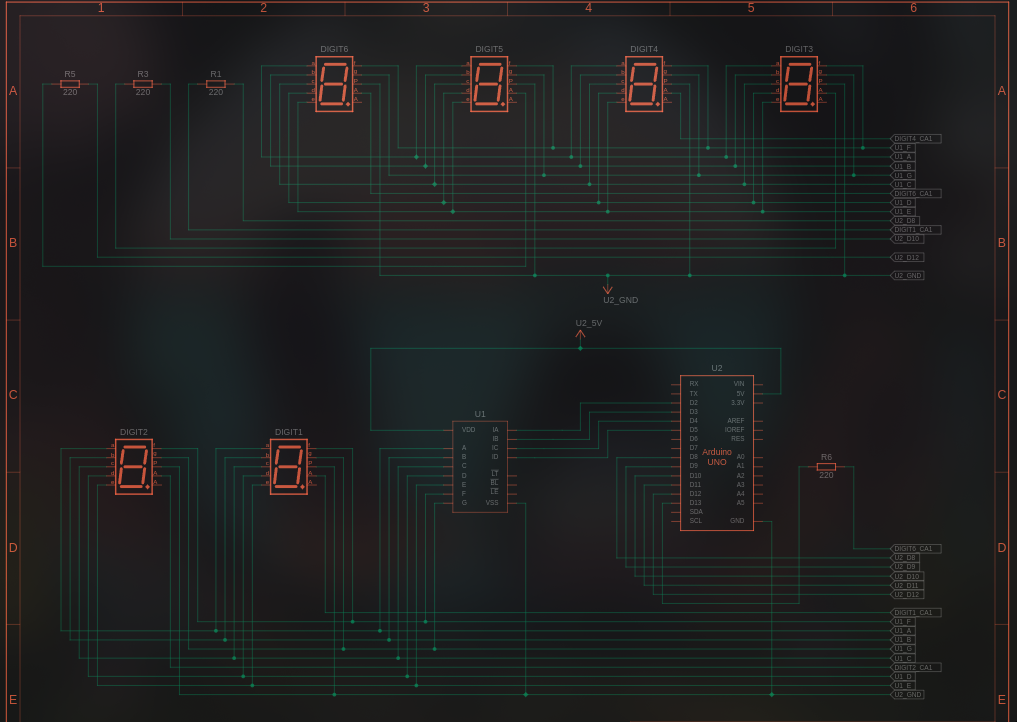
\includegraphics[width=\textwidth]{./figs/circuit_schematic.png}
    \caption{Schematic of Circuit.}
    \label{fig:circuit_schematic}
\end{figure}

\subsection*{Code implementation and Software Multiplexing}
Software Multiplexing was employed to intelligently achieve the working of 6 Seven segment displays using only one decoder.
\begin{itemize}
    \item Power pins of seven segment are connected to Digital Pins of the Arduino
    \item Data pins of all the seven segment displays are connected to the output data pins of the decoder
    \item We exploit the fact that the human eye frame rate limitations and cycle the powers of the seven segement displays at a very high rate (about $1$ ms between two digital writes) and we write to the bcd at the same time.
\end{itemize}
This multiplexing achieves the same effect as all the seven segment displays displaying the time.

\section*{Timer Initialization and Interrupt Handling}

The clock relies on precise timing through Timer1 and interrupt service routines:

\begin{verbatim}
    
void init_timer() {
    // Set CTC mode (Clear Timer on Compare Match)
    TCCR1B |= (1 << WGM12);
    
    // Set prescaler to 1024
    TCCR1B |= (1 << CS12) | (1 << CS10);

    // Set compare match value for 1s intervals (16MHz/1024)
    OCR1A = 15624;

    // Enable Timer1 compare match interrupt
    TIMSK1 |= (1 << OCIE1A);
    
    // Enable global interrupts
    sei();
}

// Interrupt Service Routine triggered every second
ISR(TIMER1_COMPA_vect) {
    flag = 1;  // Set flag to update clock values
}
\end{verbatim}

The timer operates in CTC mode with a 1024 prescaler, generating an interrupt every second. When the interrupt occurs, the ISR sets a flag that triggers the time update in the main loop, ensuring accurate timekeeping without blocking program execution.
\newline

This uses the Arduino's internal clock to achieve very minimal time losses.

\section*{Conclusion}
This project has demonstrated my attempt to implement a fully functional timer using 7 segment displays, a decoder, and an AtMega328p microcontroller (arduino uno) implemented using AVR GCC.

\end{document}
